\documentclass{beamer}

\usepackage[utf8]{inputenc}
\usepackage[polish]{babel}
\usepackage[T1]{fontenc}
\usepackage{amsfonts}
\usepackage{amsthm}
\usepackage{amsmath}
\usepackage{amssymb}
\usepackage{mathabx}
\usepackage{physics}
\usepackage{array}             
\usepackage{dsfont}
\usepackage{url}
\usepackage{wrapfig}
\usepackage{subcaption}
\usepackage{blkarray}
\usepackage{opensans}
\usepackage{float}
\usepackage{xspace}
\usepackage{xcolor}
\usepackage{hyperref}
\usepackage{algorithm}
\usepackage[noend]{algpseudocode}
\def\Z{\mathbb Z}
\def\Q{\mathbb{Q}}

\usepackage{listings}
\usepackage{ bbold }

\hypersetup{
    colorlinks=true,
    linkcolor=blue,
    filecolor=magenta,      
    urlcolor=blue,
}

%Information to be included in the title page:
\title{Problem Skolema- LATO proseminar}
\author{Marcin Wierzbiński}
\institute{MIMUW}
\date{\today}


\theoremstyle{definition}
\newtheorem*{definicja}{Definicja}
\newtheorem*{twierdzenie}{Twierdzenie}
\newtheorem*{uwaga}{Uwaga}



\begin{document}
\frame{\titlepage}

\begin{frame}{Motywacja}
\begin{itemize}
    \item Twierdzenie Skolema dla  $2$
    \item Problem Skolema
    \item 
\end{itemize}
\end{frame}
% tlumaczenie dlaczego to nie jest wykonywalna na maszynie

\begin{frame}{Zacznijmy od prostego}
    Input: 

    \begin{algorithmic}[l]
    \State $\vec{x} := \vec{a}$
    \State $\vec{a} \in \Z^{k}$
    \While { $u^{T}\cdot \vec{x} \neq 0$ }
      \State $\vec{x} := M \vec{x}$
      
    \EndWhile
    \end{algorithmic}

    Jestem zainteresowany problemem stopu dla tego problemu? To jest nieskończona pamięć, ponieważ $x$ może rosnąć bardzo dużo
    Czy jest rozstrzygalny ten program? To twierdzi inaczej?


\end{frame}

\begin{frame}{Pytanie o inny warunek}
    Zmieńmy warunek na inny 
    \begin{algorithmic}[l]
    \State $\vec{x} := \vec{a}$
    \State $\vec{a} \in \Z^{k}$
    \While { $u^{T}\cdot \vec{x} \geq 0$ }
      \State $\vec{x} := M \vec{x}$
      
    \EndWhile
    \end{algorithmic}
\end{frame}    

\begin{frame}{Inne pytanie z terminów automatów}
    Mamy alfabet $\Sigma$  oraz A, B skończony automat deterministyczny lub nie-deterministyczny nad alfabetem $\Sigma$
    \begin{itemize}
        \item $u_n$ numer slów długości $n$ akceptowanych przez $A$
        \item  $v_n$ jest numerem slow długości $n$ akceptowanych przez automat $B$

    \end{itemize}
    Pytanie:
    $\exist n = u_n = v_n$
    lub inne 
    $\forall v_n \leq u_n$
    Ten problemy nie jest są znane jako rozstyrzgalne i nie są nierostrzygalne
    I sa redukowane do problemu 1
    Znana jest rozstrzygalnosc dla automatow autoamtow rozmiaru $4$

\end{frame}

\begin{frame}{Równoważność pytania}
    \begin{figure}
        \centering
        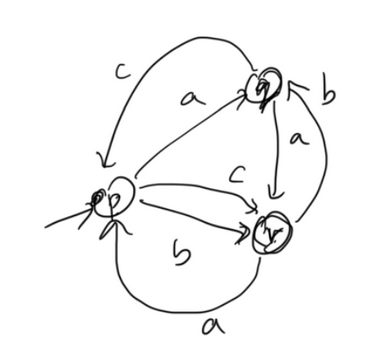
\includegraphics[width=40mm]{img/Zaznaczenie_079.png}
        \caption{Automat skończony}
        \label{fig:my_label}
    \end{figure}
    \begin{cases}
        p_{n+1} = r_n + g_n \\
        g_{n+1} = p_n + r_n \\ 
        r_{n+1} = 2 p_n + q_n \\ 
        (p_0, q_0, r_0) = (1,0,0) 
    \end{cases}
\end{frame}

\begin{frame}{Liniowe równanie rekurencyjne}
    $$
        a_0, \ldots a_{k-1} \in \mathbb{Z} 
    $$

    $$
        u_0, \ldots, u_{k-1} \in \mathbb{Z}
    $$


    Liniowe równanie rekurencyjne: 
    $$
    u_{n+k}=a_{1} u_{n+k-1}+a_{2} u_{n+k-2}+\ldots+a_{k} u_{n}
    $$
    Zwykłe oznaczenie $<u_n>_{n=1}^{\infty}$
    $a_0 \neq 0$
\end{frame}

\begin{frame}
    Przykad:
    Równanie Fibonacciego:
   \begin{equation*}
        \begin{cases}
        u_{n+2} = u_{n+1} + u_n \\
        u_{1} = 1 \\
        u_{0} = 0
        \end{cases}
    \end{equation*}
    Jest bliska styczność z przykładami wyżej. 

\end{frame}

\begin{frame}{Zapis macierzowy}
    $$\exist v, w \in \mathbb{Z}^{k}, M \in \mathbb{Z}^{k\times k} $$
    $u_n = v^{t}M^{n}w$

    $$
    M = \begin{bmatrix}
    a_{k-1} & 1 &  \ldots & 0 \\
    a_{k-2} & 0 & 1 & \ldots 0  \\
    \vdots & 0 & \ldots & 0 \\ 
    a_1 & 0 & \ldots & 1 \\
    a_0 & 0 & \ldots & 0
    \end{bmatrix}
    $$
\end{frame}

\begin{frame}{Lemat redukcji}

\begin{theorem}{Cayley-Hamiltonian}
    Jeśli $p(t)$ jest wielomianem charakterystycznym dla macierzy $M$, wtedy macierz $p(M)$ jest macierzą zerową. 
\end{theorem}

\begin{theorem}

    Niech $v, w \in \mathbb{Z}^{k}, M \in \mathbb{Z}^{k\times k}$.
    Niech $u_n = v^{t}M^{n}w \in \mathbb{Z}$
    Wtedy $<u_n>$ jest liniowym równaniem rekurencyjnym. 

\end{theorem}



\begin{proof}
    Weźmy $M$ wówczas z twierdzenia CH: 
    $$M^{k} a_1 M^{k} + \ldots a_0 \mathbb{1}$$ 
    może to równanie przez 
    $$ v^{t}M^{k} = a_1 v^{t} M^{k-1} + \ldots a_k v^{t} \mathbb{1}$$ 
\end{proof}

\end{frame}

\begin{frame}{lemat c.d}
i pomnażam przez $M^{n}$ z lewej strony 
      $$ v^{t}M^{k} M^{n} = a_1 v^{t} M^{k-1} M^{n} + \ldots a_k v^{t} \mathbb{1} M^{n}$$ 
      i pomnażam 
      $$ v^{t}M^{k} M^{n} w = a_1 v^{t} M^{k-1} M^{n}w + \ldots a_k v^{t} M^{n}w $$ 
      co daję tezę
\end{frame}

\begin{frame}{Lemat w drugą stronę}
\begin{theorem}
    Niech $<u_n>$ bedzie równaniem lin. rekurencyjnym z początkowymi zmiennymi $u_0, \ldots u_{k-1}$. 
    Niech
    $$
    M = \begin{bmatrix}
    a_{1} & 1 &  \ldots & 0 \\
    a_{2} & 0 & 1 & \ldots 0  \\
    \vdots & 0 & \ldots & 0 \\ 
    a_{k-1} & 0 & \ldots & 1 \\
    a_{k} & 0 & \ldots & 0
    \end{bmatrix}
    $$

    $$v= \begin{bmatrix}
    u_{k-1} \\ u_{k-2} \\ \vdots \\ u_{0} \\
    \end{bmatrix}
    w =  \begin{bmatrix}
    0 \\ 0 \\ \vdots \\ 1 \\
    \end{bmatrix}
    $$
    pokaż, że $u_n = v^{t} M^{n} w$
\end{theorem}
\begin{proof}
    Przez indukcje
\end{proof}
\end{frame}

\begin{frame}{Równanie fib:}

\begin{equation*}
\begin{cases}
u_{n+2} = u_{n+1} + u_n \\
u_{1} = 1
u_{0} = 0
\end{cases}
\end{equation*}

        \begin{bmatrix}
        1 & 1\\
        1 & 0
        \end{bmatrix}^n
        = 
        \begin{bmatrix}
        u_{n+1} & u_n\\
        u_{n} & u_{n-1}
        \end{bmatrix}
\end{frame}

\begin{frame}{Bogactwo innych przykładów}
Równanie rekurencyjne Fibonacciego: 
$$
{\displaystyle u_{n}={\frac {1}{\sqrt {5}}}\left({\frac {1+{\sqrt {5}}}{2}}\right)^{n}-{\frac {1}{\sqrt {5}}}\left({\frac {1-{\sqrt {5}}}{2}}\right)^{n}.}
$$

    $u_n = n$
    Jak zapisać za pomocą równania rekurencyjnego? 
    $u_n = n^{2}$
\end{frame}

\begin{frame}{$u_n = n^{2}$}
    $u_{n+3} = 3 u_{n+2} - 3 u_{n+1} + u_{n} $
\end{frame}

\begin{frame}{Problem Skolema dla równania rzędu 2}
    $u_n$ jest równaniem rekurencyjnym liniowym rzędu 2
    $$
        u_n = c_1 u_{n+1} + c_2 u_n
    $$
    $$
        c_1, c_2 \in \mathbb{Q}
    $$
    $$
        u_0, u_1 \in \mathbb{Q}
    $$
    
    $\exist n : u_n = 0 ?$
\end{frame}

\begin{frame}{Szkic dowodu}
    
    $$
        x^{2} - c_1 x - c_2 = 0
    $$
    $$ 
        \lambda_1, \lambda_2 \in \hat{\Q}
    $$
    rozpatrzymy pierwszy przykład:
    $\lambda_1 \neq \lambda_2$
\end{frame}

\begin{frame}{Przykład:}
\begin{itemize}
   \item  Rozważmy ciąg: 
   \item  $$ 0, 0, 1, 0, 1, 0, 2, 0, 3, 0, 5, 0, 8, 0, ...$$
    \item      Zauważmy szereg Fibonacciego pomiędzy zerami. 
    \item  Zdefiniowany takim wzorem:
    \item  $F(i) = F(i-2) + F(i-4)$
    \item  Startując od przypadku podstawowego $F(1) = F(2) = F(4) = 0$i $F(3) = 1$
    \item  Wówczas $F(i) = 0 \iff \text{i jest 1 lub parzyste} $  
    \item pozycje na którym mamy zero możemy podzielić na singleton ${1}$ zbiór skończony i ciąg pełnie arytmetyczny ciąg parzystych liczb. 
\end{itemize}
\end{frame}

\begin{frame}{Dowód  SML}
    Niech $$u_{n+k}=a_{1} u_{n+k-1}+a_{2} u_{n+k-2}+\ldots+a_{k} u_{n}$$

    Załóżmy, że $a_o \neq 0$, wówczas $\exist v, w, M$ takie, że 
    $u_n = u^{t} M^{n} w $ wszystko nad $\mathbb{Z}$

    Wyznacznik $det(M) = \pm a_0 \neq 0$
    Wybierzmy liczbę pierwsza $p > 2$ t,że $p \nmid a_0$
\end{frame}

\begin{frame}{dowód c.d}
    Rozważmy $M_p \in \mathbb{F}_p^{k\times k} $, $det(M_p) \neq 0$
    Jest takich co najwyżej $p^{k^{2}}$
\end{frame}

\begin{frame}{Przykłąd}
Problem 1 jest znany jako problem Skolema 
    $\left\{n \in \mathbb{N}: u_{n}=0\right\}$
\end{frame}

\begin{frame}{Wielomian charakterystyczny}
    $u_{n}=p_{1}(n) \gamma_{1}^{n}+\ldots+p_{k}(n) \gamma_{k}^{n}$
    $p_{1}, \ldots, p_{k} \in \mathbb{C}[x]$
\end{frame}

\begin{frame}{Ultimate Positivity Problem}
    Własnośc stopu dla programu

\end{frame}



\begin{frame}{Skolem problem}
    Czy dane liniowe rekurencyjne ma zero. 
    $u_n = 0$ dla pewnego $n$?
    \begin{itemize}
        \item Istnieje algorytm pozwalający sprawdzić, czy istnieje nieskończona ilość zer, a jeśli tak, to znaleźć rozkład tych zer na zbiory okresowe, gwarantowane przez twierdzenie Skolema-Mahlera-Lecha. 
        \item Nie wiadomo jednak, czy istnieje algorytm pozwalający określić, czy sekwencja rekurencyjna ma jakieś nieperidoczyne zera. 
    \end{itemize}
\end{frame}


\begin{frame}


\begin{itemize}
    \item https://terrytao.wordpress.com/2007/05/25/open-question-effective-skolem-mahler-lech-theorem/
\end{itemize}
\end{frame}

\end{document}